\documentclass[paper=a4, english, ngerman, romanian]{scrartcl}

\usepackage[a4paper,left=2cm,right=2cm,top=2.5cm,bottom=3cm]{geometry}
\usepackage[ngerman]{babel}
\usepackage{tabularx}
\usepackage[utf8]{inputenc}
\usepackage{multirow}
\usepackage{listings}
\usepackage{graphicx}

\parindent 0pt
\lstset{basicstyle={\ttfamily\scriptsize}, tabsize=4}

\title{Datenbanksysteme SS17: Projekt}
\author{Bernadeta Chisarau, Dor Cohen, Mihai Renea}

\begin{document}

	\maketitle
	
	\pagebreak
	
	\section{Datenalanlyse}
		Der Datensatz erfasst mehr als 6000 Tweets von dem Wahlkampf zwischen den Kandidaten für US-Präsident Donald Trump und Hillary Clinton. Der Datensatz entsteht aus den folgenden Feldern:
		\begin{enumerate}
		\item \textit{handle} - Der Autor des Tweets
		\item \textit{text} - der Inhalt
		\item \textit{is\_retweet} - Markiert, ob es ein Retweet ist
		\item \textit{original\_author} - Falls Retweeted, der originale Autor
		\item \textit{time} - Das Time-Stamp des Tweets (Datum und Uhrzeit)
		\item \textit{in\_reply\_to\_screen\_name} - Der Name der Person, für die das Tweet eine Antwort sein soll (inkonsistent)
		\item \textit{is\_quote\_status} - ?
		\item \textit{retweet\_count} - Anzahl der Retweets von einem Tweet
		\item \textit{favorite\_count} - Anzahl der Likes
		\item \textit{source\_url} - Warscheinlich die Quelle des Tweets
		\end{enumerate}
		
		Manche der obengenannten Feldern werden wir nicht in Betracht ziehen, weil sie irrelevant für unsere Zwecke, inkonsistent oder mangelhaft sind:
		
		\begin{itemize}
		\item \textit{original\_author} werden wir Ignorieren, da nur eine Name keine interessante Information uns geben kann. \textit{is\_retweet} werden wir aber behalten, da es eine Rolle bei der Funktion der Wichtigkeit von Tweets eine Rolle spielen könnte.
		\item \textit{in\_reply\_to\_screen\_name} kann weggelassen werden, da es inkonsistent und scheinbar fehlerhaft erzeugt wurde (z.B. in der Mehrheit der Fällen, wo dieser Feld auftritt, antwortet Hillary Clinton sich selbst).
		\item  In \textit{is\_quote\_status} konnten wir keine Schablonen erkennen, deshalb liefert das uns nichts nutzbares.
		\item \textit{source\_url} ist irrelevant.
		\end{itemize}
		
		Andere Informationen sind aber von besonderer Wichtigkeit für unseren Zweck:
		
		\begin{itemize}
		\item \textit{time} wird uns helfen die Entwicklung der Hashtags-Nutzung über die ganze Zeit zu analysieren. 
		\item \textit{retweet\_count} und \textit{favorite\_count} werden die Schlüsselargumente fur die Modellierung der Funktion der Wichtigkeit von Tweets sein.
		\end{itemize}
	
	Die folgende MinMax-Diagramm stellt das ER-Modell vor. Die Attributen \textit{Time Stamp} werden von dem Composite-Attribut \textit{Time Stamp} hergeleitet.
	
	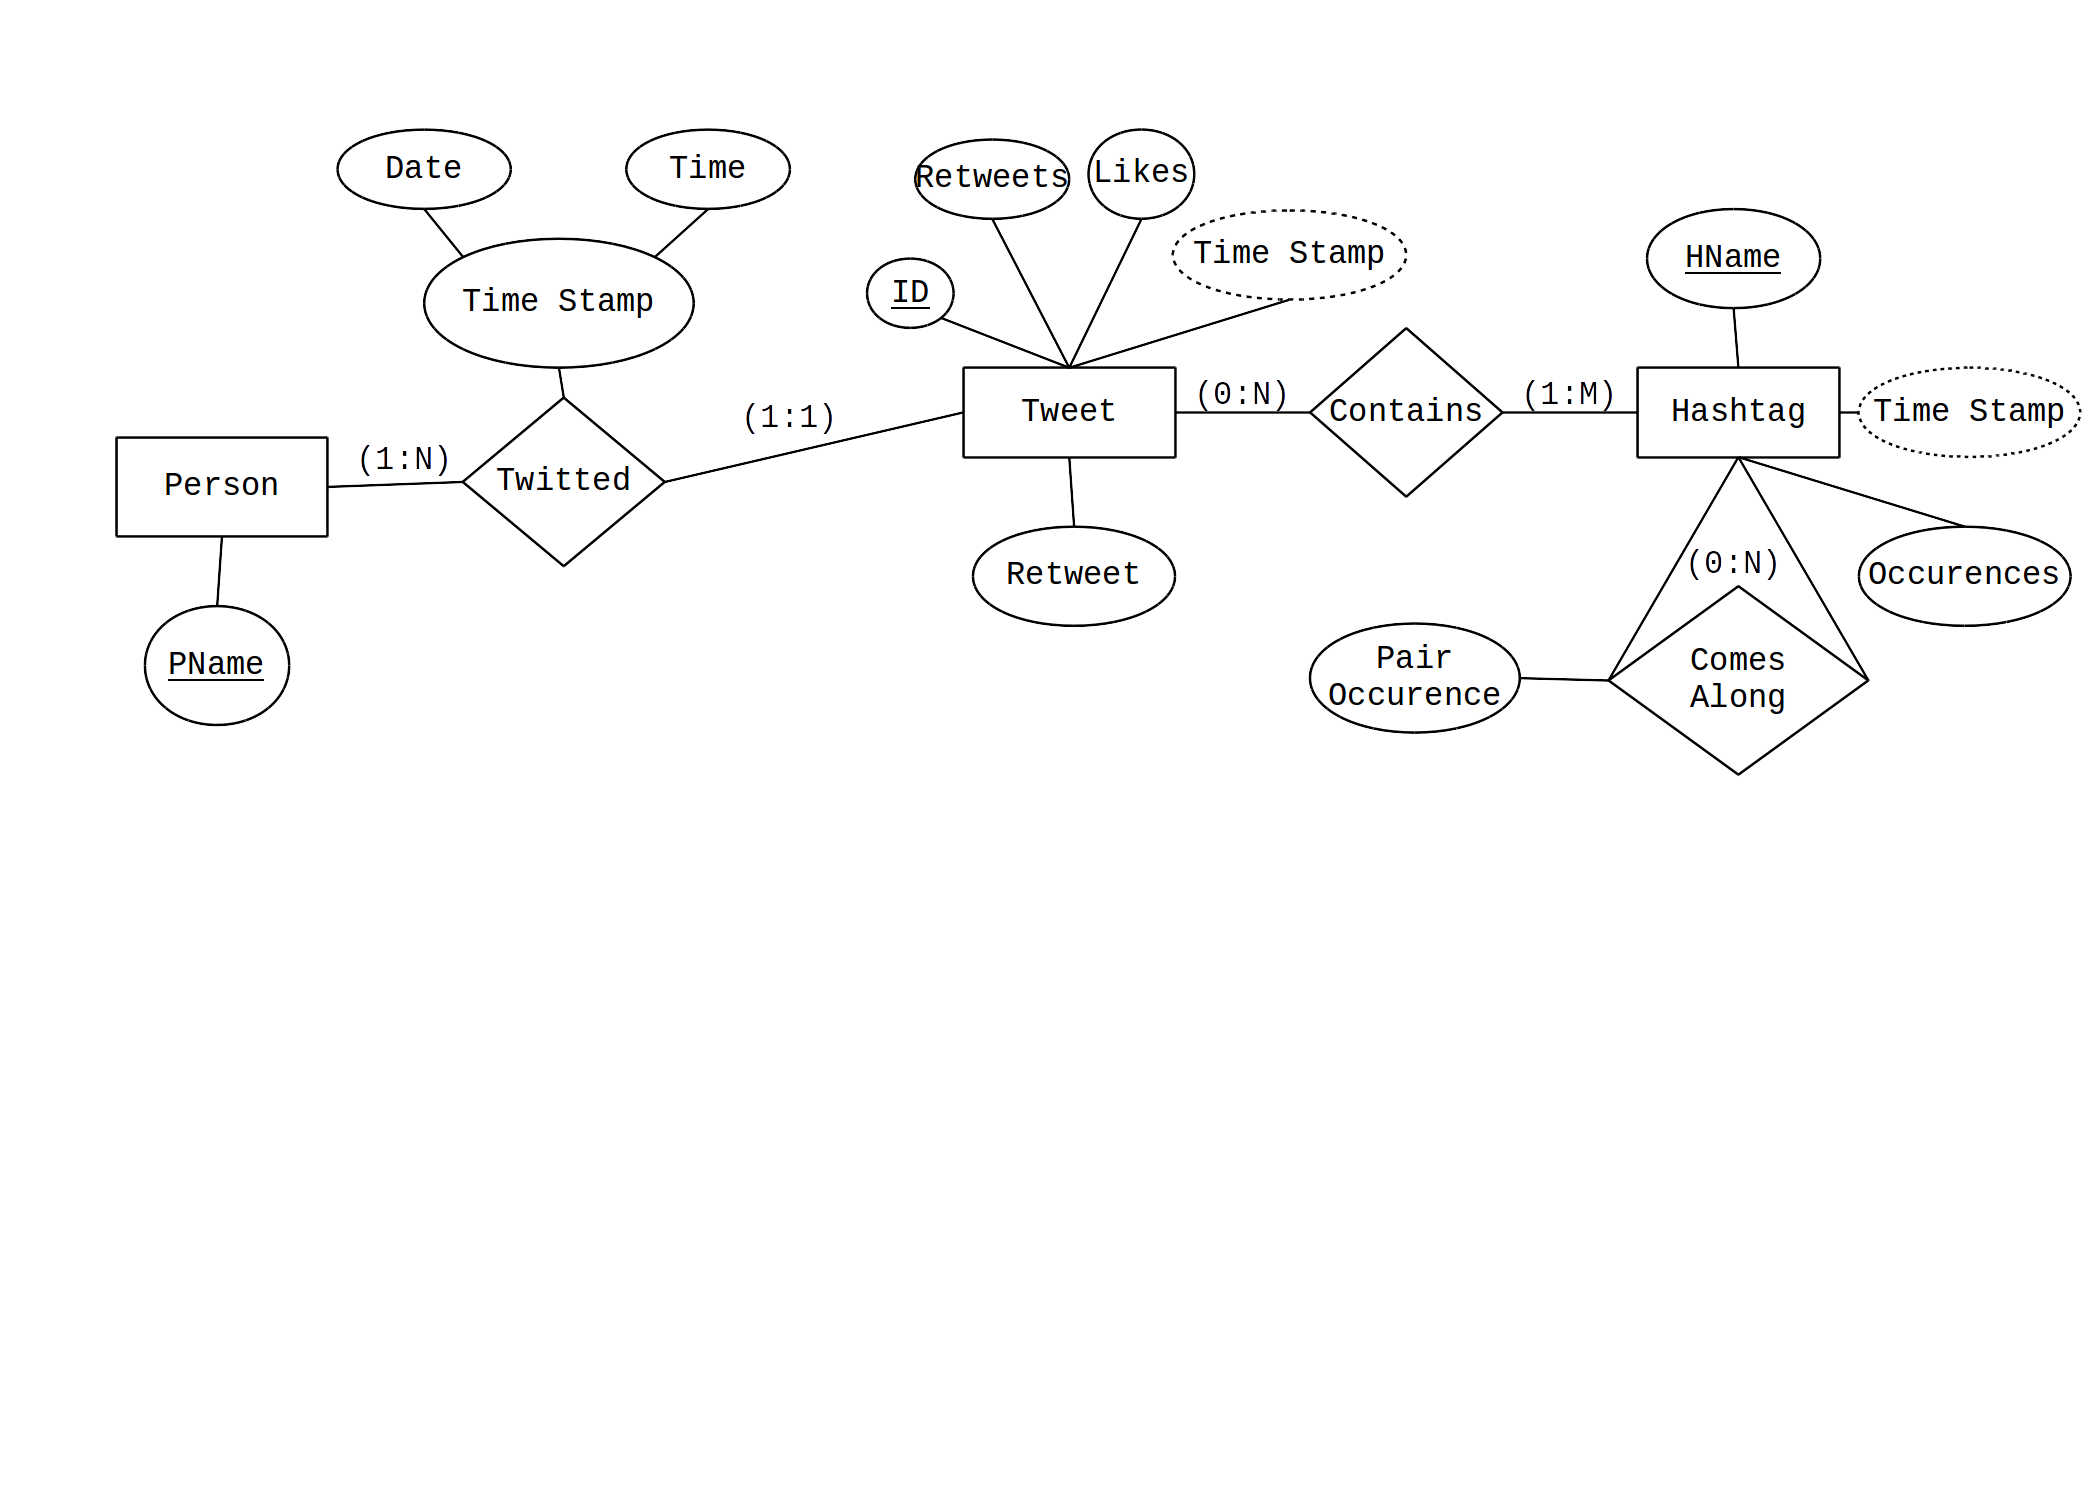
\includegraphics[scale=0.8]{MinMax_Diagram.png}

\begin{center}
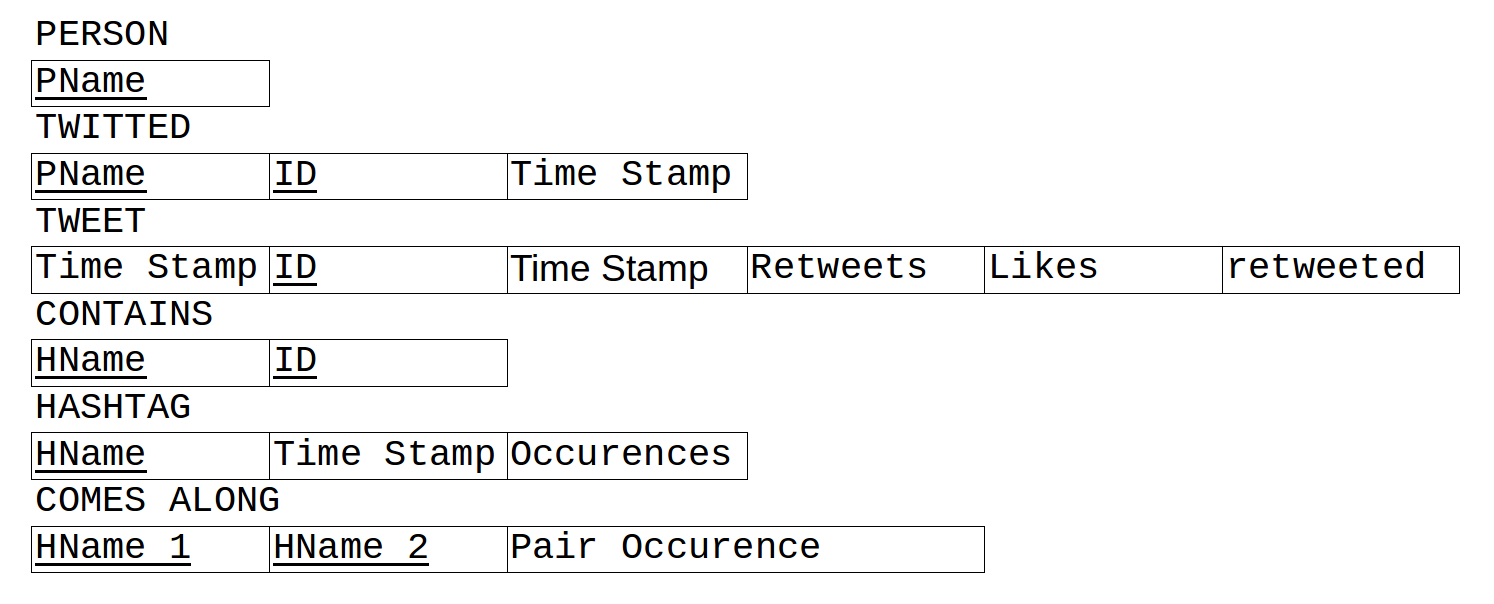
\includegraphics[scale=0.25]{Screenshot_2017-05-08_21-17-03}
\end{center}
	

\end{document}
